
%%%%%%%%%%%%%%%%%%%%%%% file typeinst.tex %%%%%%%%%%%%%%%%%%%%%%%%%
%
% This is the LaTeX source for the TDPTemplate using
% the LaTeX document class 'llncs.cls' Springer LNAI format
% used in the RoboCup Symposium submissions.
% http://www.springer.com/computer/lncs?SGWID=0-164-6-793341-0
%
% It may be used as a template for your own TDP - copy it
% to a new file with a new name and use it as the basis
% for your Team Description Paper
%
% NB: the document class 'llncs' has its own and detailed documentation, see
% ftp://ftp.springer.de/data/pubftp/pub/tex/latex/llncs/latex2e/llncsdoc.pdf
%
%%%%%%%%%%%%%%%%%%%%%%%%%%%%%%%%%%%%%%%%%%%%%%%%%%%%%%%%%%%%%%%%%%%

\documentclass[runningheads,a4paper]{llncs}
\usepackage{amssymb}
\setcounter{tocdepth}{3}
\usepackage{graphicx}
\usepackage{amssymb}
\usepackage[utf8]{inputenc}
\usepackage{url}
\usepackage{float}
\usepackage{amsmath}
\usepackage{graphicx}
\usepackage{wrapfig}
\usepackage{subfigure}

% *** MORE GRAHPICS ***
\usepackage[usenames,dvipsnames]{color}     

% *** BIBLIOGRAPHY PACKAGES ***
%\usepackage{natbib}     

%%%%%%%%%%%%%%%%%%%%%%%%%%%%%%%%%%%%%%%%%%%%%%%%%%%%%%%%%%%%%%%%%%%
\usepackage{booktabs}           % For tables (toprule, midrule, bottomrule)
%%%%%%%%%%%%%%%%%%%%%%%%%%%%%%%%%%%%%%%%%%%%%%%%%%%%%%%%%%%%%%%%%%%

%%%%%%%%%%%%%%%%%%%%%%%%%%%%%%%%%%%%%%%%%%%%%%%%%%%%%%%%%%%%%%%%%%%
% *** PATHS ***
\makeatletter
\def\input@path{{figures/}		
			   }
\makeatother

\graphicspath{{figures/}
			 }
%%%%%%%%%%%%%%%%%%%%%%%%%%%%%%%%%%%%%%%%%%%%%%%%%%%%%%%%%%%%%%%%%%%

%%%%%%%%%%%%%%%%%%%%%%%%%%%%%%%%%%%%%%%%%%%%%%%%%%%%%%%%%%%%%%%%%%%
\newcommand{\eg}{\emph{e.g.}}						% Exemplum gratia
\newcommand{\ie}{\emph{i.e.}}						% Id est
%%%%%%%%%%%%%%%%%%%%%%%%%%%%%%%%%%%%%%%%%%%%%%%%%%%%%%%%%%%%%%%%%%%

\begin{document}

\title{RoboFEI @Home 2016 Team Description Paper}
\author{Andrey~A.~Masiero, Leonardo~Contador, Lucas~Vasconcelos, Flavio~Tonidandel and Plinio~T.~Aquino~Junior}
\institute{Centro Universitário FEI,
\newline Av. Humberto Alencar de Castelo Branco, 3972, 09850-901, SBC, SP, Brazil\\
\texttt{http://www.fei.edu.br/robofei, amasiero@fei.edu.br}}
\authorrunning{A.A.~Masiero et al.}

%\author{Team Leader \and Team Members }
%\institute{[Intitute name and direction here], \\
%\texttt{http://devoted-web-site.url}}
\maketitle


%%%%%%%%%%%%%%%%%%%%%%%%%%%%%%%%%%%%%%%%%%%%%%%%%%%%%%%%%%%%%%%%%%%%%%%%%%%%%%%%%%%%

\begin{abstract}
%In your abstract, please state which is the main research line of your team for this year (on which problem or set of problems are you focusing all the team efforts). Tell why this research is important, how are you approaching to the problem solution and which results do you expect to obtain.
This paper provides an overview of the developments of the RoboFEI @Home team in the last year. ToDo: update. The main research effort of the past year has focused on developing a global, volumetric, object-oriented world model. This world model should replace all world representations that are commonly present in an architecture, e.g., for navigation and manipulation. As a result, these modules can benefit from the additional knowledge that is present in the world model. This world modeling approach is expected to i) make modules such as navigation more robust since these can benefit from the additional knowledge that is present in the world model and ii) reduce the amount of hardcoded knowledge that is commonly present. 
\end{abstract}


%%%%%%%%%%%%%%%%%%%%%%%%%%%%%%%%%%%%%%%%%%%%%%%%%%%%%%%%%%%%%%%%%%%%%%%%%%%%%%%%%%%%

\section{Introduction}
%\section{Introduction}

This paper describes the hardware and software aspects of the RoboFEI@Home team, designed to compete in the RoboCup 2016 @Home League.

The first steps towards the first group of research in robots at Centro Universitário da FEI was made by Prof. Reinaldo Bianchi in 2002 with the first groups of students in RoboCup Simulation 2D. Next year, with the experience of Prof. Reinaldo Bianchi who have participated in the soccer robot group in USP since 1998, together with Prof. Flavio Tonidandel, developed the first robots for Very Small Size Category of the IEEE Robotic Competition. In 2004, during the First Brazilian Competition on Intelligent Robots (a competition in which the IEEE Robot Competition was held together with the First Brazilian RoboCup), our team became Brazilian Champion in the IEEE Very Small category. In the same competition, our first team developed for the RoboCup Small Size League became vice-champion In 2006, Very Small Size team became Champion again, and our first 2D RoboCup Simulation team was the Brazilian champion.

The institution RoboCup Small Size League team, called RoboFEI, won for the first time the Brazilian Robocup in 2010, and is currently the Brazilian champion, winning the championship 6 times in a row (2010, 2011, 2012, 2013, 2014 and 2015). This team takes part in the RoboCup World Competition since 2009, and the best result we had was in 2012, when we stayed among the top 8 teams. After developing robotic soccer players for the last 17 years, we developed a team to compete in the RoboCup Humanoid League. The development of this team started in 2012, with students designing and building a humanoid robot from scratch. Last year, the RoboFEI-HT team competed our first RoboCup World Competition, held in João Pessoa, PB, Brazil, with 4 humanoid robots: two Newton (developed in-house, being the pieces of one of them, made in a 3D printer) and two humanoids robots based on Darwin-OP. At RoboCup 2014, the team stayed among the 16 top teams and in the same year, the team competed the Latin American Robotics Competition (LARC 2014) and became champion in the LARC RoboCup Humanoid Kid Size league.

Now that the institution has establish important positions on small size and humanoid league, we decide to drive our research into new paths for collaborating on social and service robots. The robot design, particularly the human factor concerns, are a key aspect of human-robot interaction (HRI). Research in HRI attractions from similar research in human-computer interaction (HCI) but features a number of significant differences related to the robot’s physical real-world personification. This team was born in Usability Engineering Laboratory, now defined as Human Robot Interaction and Intelligent Interfaces Group (HR3iGroup). This research group has abundant knowledge in HCI and is focused on integrating with HRI. The robot’s physical personification, simplicity or complexity of design, form and level of anthropomorphism, human behavior and robot interaction feedback, robotic reactions and humanized relationships, are some of the key research areas being explored.

Last year, we applied for and achieved 3rd place at the Latin American @Home competition. We focus on research applied in Human-Robot Interaction, Social and Service Robots, Behavior Analysis, People Modeling and Profiling, and all questions for improving people and robots coexistence.


%\section{World Modeling}\label{oo:sec:ed}
%\input{ed.tex}
%
%\section{Perception}\label{sec:perception}
%\input{perception.tex}
%
%\section{Navigation}\label{sec:navigation}
%\input{navigation.tex}

\section{Conclusions}
%We have described all development of our robot Judith. We believe that all of these tasks can help on home, health and office services. To improve the acceptance of these robots, we have been working into a behavior analysis framework developed using ROS. With this framework, we pretend:
\begin{itemize}
    \item Identifying people's emotion;
    \item Creating user behavior profile;
    \item Improving approach to start a interaction.
\end{itemize}
With this TDP, we hope to participate on Robocup 2016 in Germany and try to advance during the competition and learning with all teams, as we did to win third place on XIV Latin American Robotic Competition in 2015. Hope see you all there.

\section*{Robot Hardware Descriptions}
%\section{Hardware Design}

Our team has one robot, called Judith (see Fig.~\ref{fig:judith}). Judith is a robot based on the Peoplebot platform~\cite{peoplebot:2001}, using a KUKA youBot arm~\cite{youbot:2016} as its main manipulator. As shown in Fig.~\ref{fig:judith}, Judith is composed of: 1 Microsoft Kinect for Xbox 360; 2 sonar arrays; 2 infrared sensors; 1 iPad 2; 1 Yoga HT-320A microphone; 1 touch sensor arrays; 2 speakers; 1 emergency button; and 1 Hokuyo URG-04LX-UG01 laser sensor.

Peoplebot has a vertical grip which was removed for the KUKA youBot arm to be attached. To attach the new arm, we built a support to keep it on the right height to manipulate objects on top of an ordinary sized table. KUKA youBot arm weighs 16.53 pounds so a wooden support was made to hang up with this weight.

\begin{figure}[ht!]
    \centering
    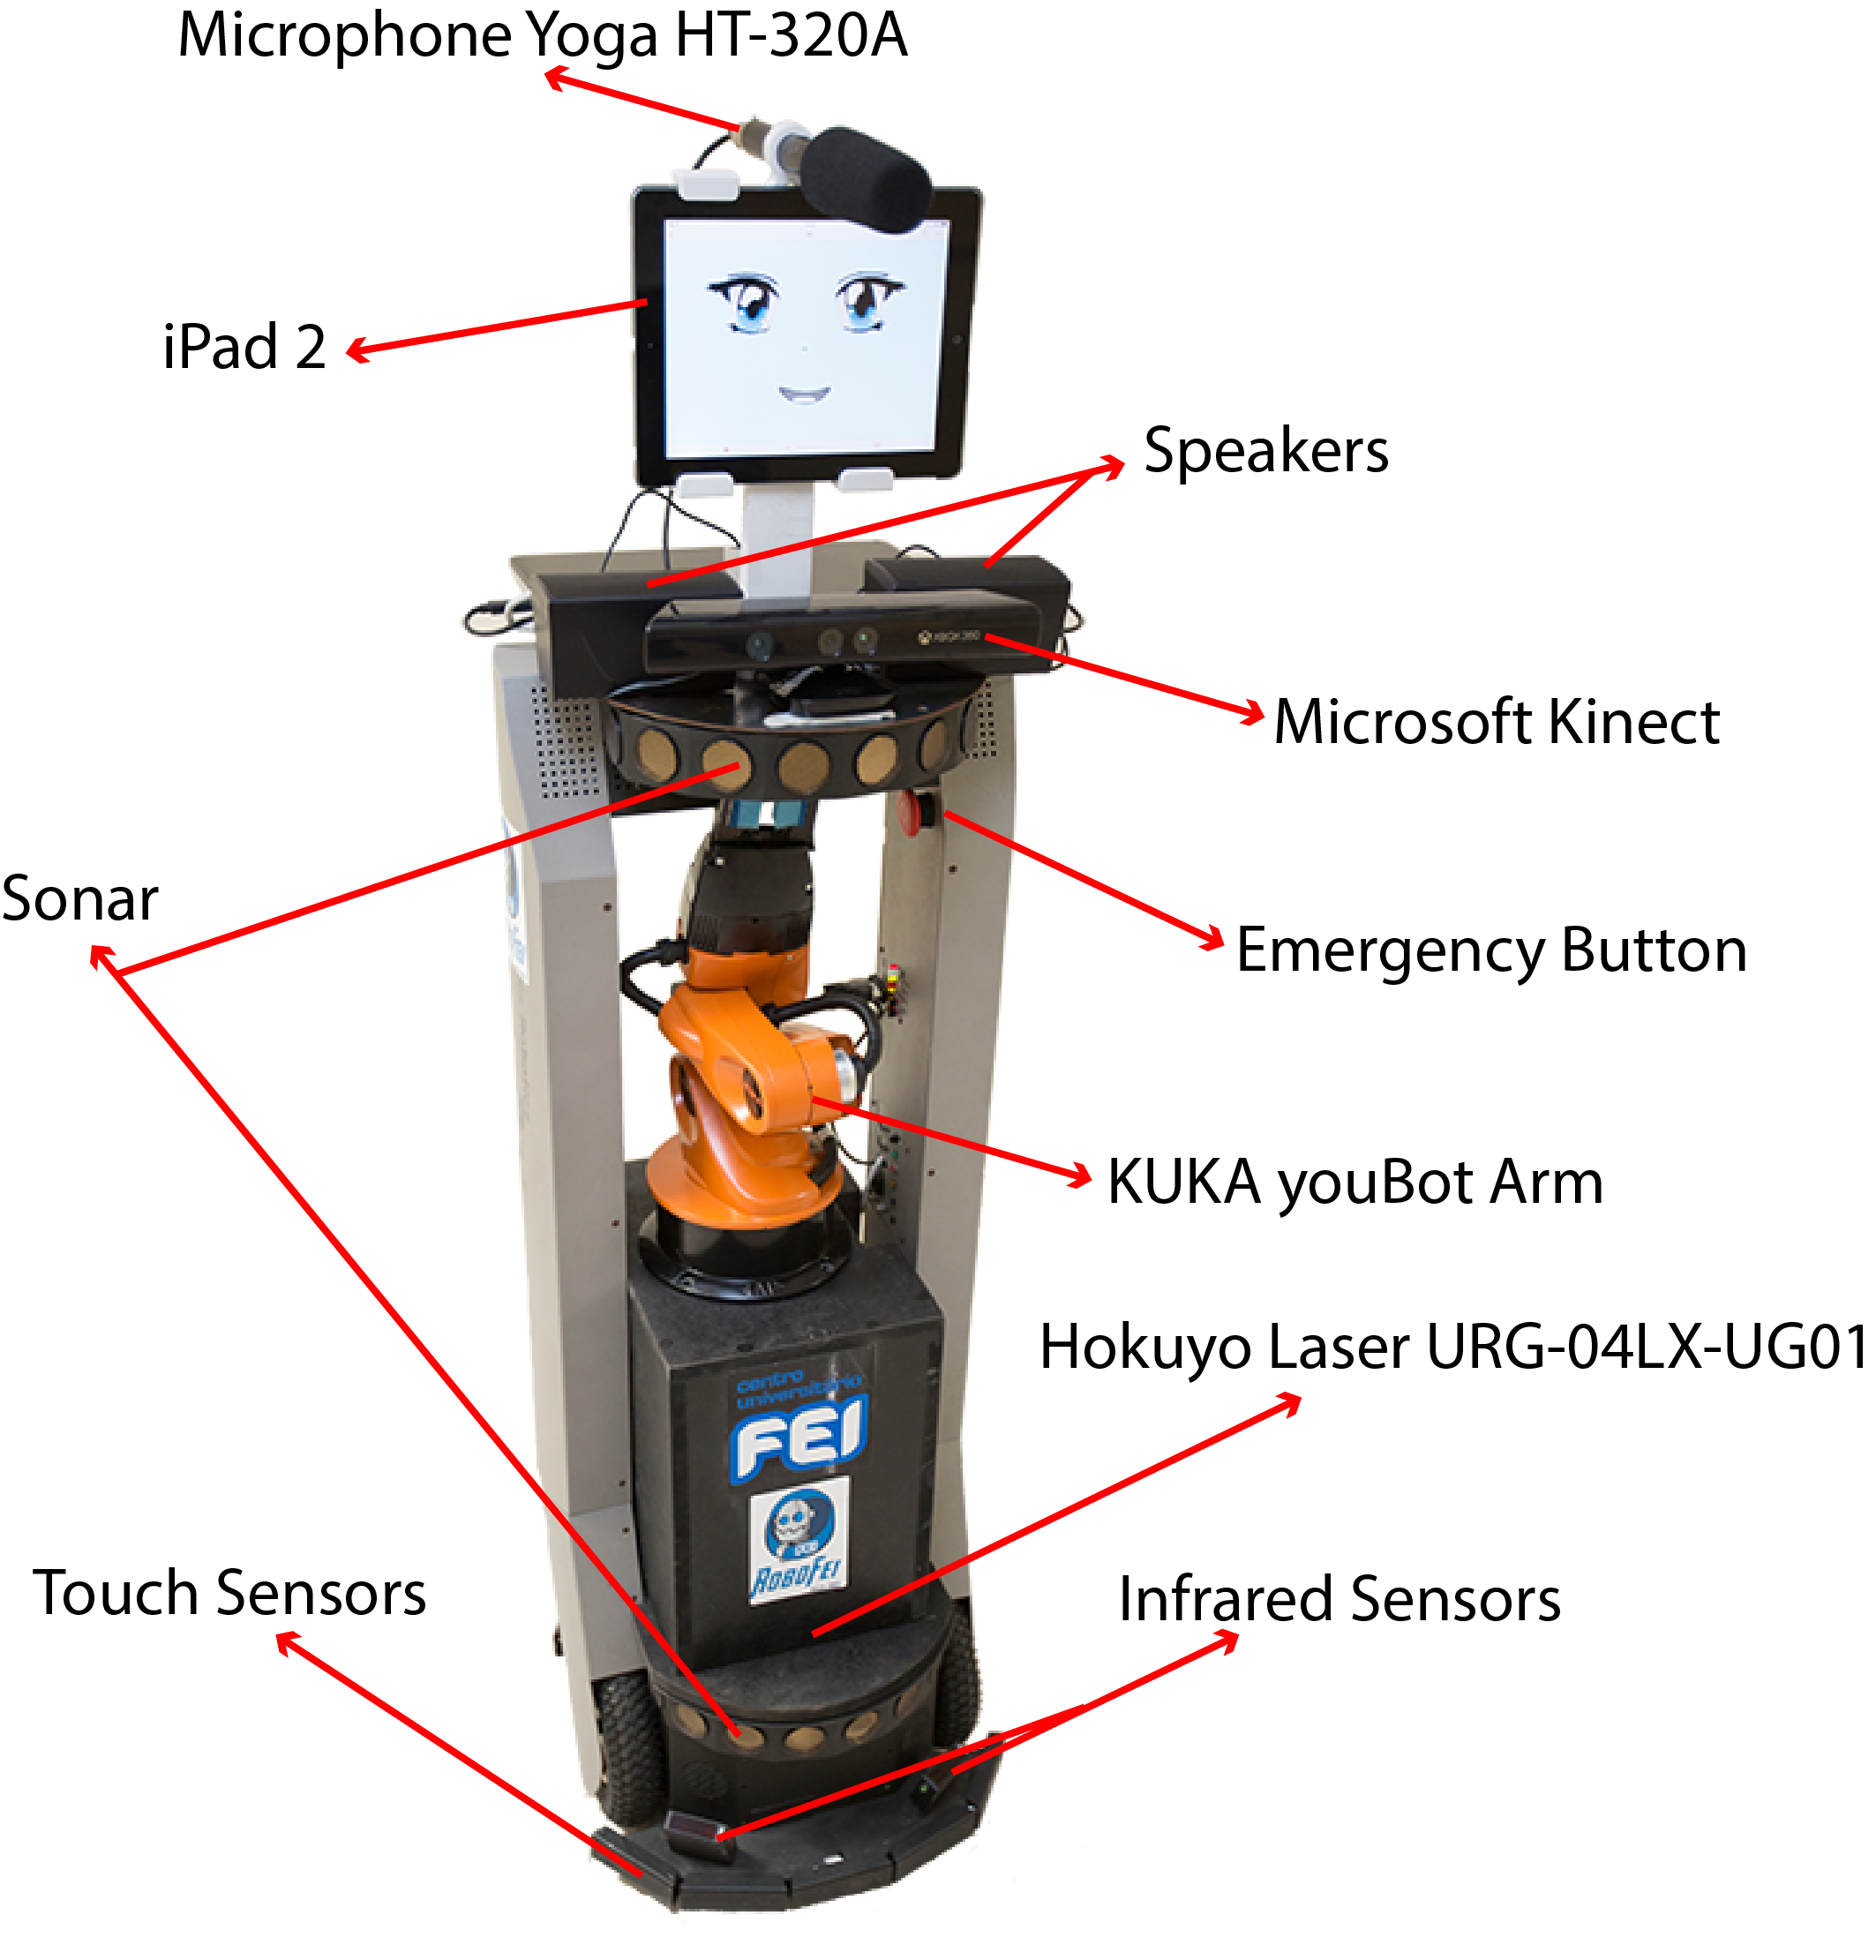
\includegraphics[height = 7.2cm]{figures/judith_info.png}
    \caption{RoboFEI's Judith}
    \label{fig:judith}
\end{figure}

Working with two different pre-manufactured robots present some challenges. First of all, each one have electric source with different voltage. KUKA youBot arm needs 24v to work while Peoplebot works with 12v. To put Peoplebot and KUKA youBot arm together, we need to build a circuit for connecting both battery kits together. This circuit is important to keep all parts of the robots safe in case of electric damage on overcharge. It also helps to make both robots work at the same time.

With both mechanical and electrical projects setups, we need to connect both robots on main computer. In order to connect Peoplebot to our laptop we used a serial RS232 to USB converter. The manipulator is able to transmit messages through an EtherCAT cable, which is connected to the computer's network port.

The robot's main computer has been an ASUS Ultrabook 14'' Touch-Screen Laptop, with an Intel Core i5, 4GB Memory, 500GB Hard Drive. It has only 3 USB ports supporting all devices, so an USB hub is used to enable more ports and increase the number of interfaced devices. As the iPad needs a paid annual license for software development, a change is being made towards Android technology so as to allow us to develop an interactive face for Judith.

The platform used by Peoplebot makes transportation a challenge, so we have worked on a modular platform using a combination of 3D print technology and aluminum parts. We want to accomplish this project until RoboCup 2016 in Germany.


\section*{Robot Software Description}
%\section{Software Design}

This section presents all details about RoboFEI@Home software. A stable version of the software is available on GitHub\footnote{\url{https://github.com/OpenFEI/rfh\_judite}}. The section is divided as: (I) Judith's software architecture; (II) face and people recognition; (III) object detection; (IV) speech recognition and synthesis; (V) navigation; (VI) object manipulation.

\subsection{Software Architecture}\label{architecture}
All of Judith's software is developed under Ubuntu Linux 14.04 LTS~\cite{sobell:2014} and ROS Indigo Igloo~\cite{ros:2015}. The initial architecture of Judith is composed by three layers. Each layer is responsible for one part of the code. The first layer receives all data from sensors, extract the features and publish it for AI and Controller nodes (Second Layer). AI and Controller nodes use the features to run algorithms for computer vision, location, planning, pattern recognition, among others. The second layer then sends to the third layer information regarding the movement of the robot, that is, the velocity of the motors, positions or velocity of the manipulator joints and face expressions to display on the iPad. The third layer controls all the actuators drivers and actions. A graphic view of the architecture is presented on Fig.~\ref{fig:architecture}.

\begin{figure}[ht!]
    \centering
    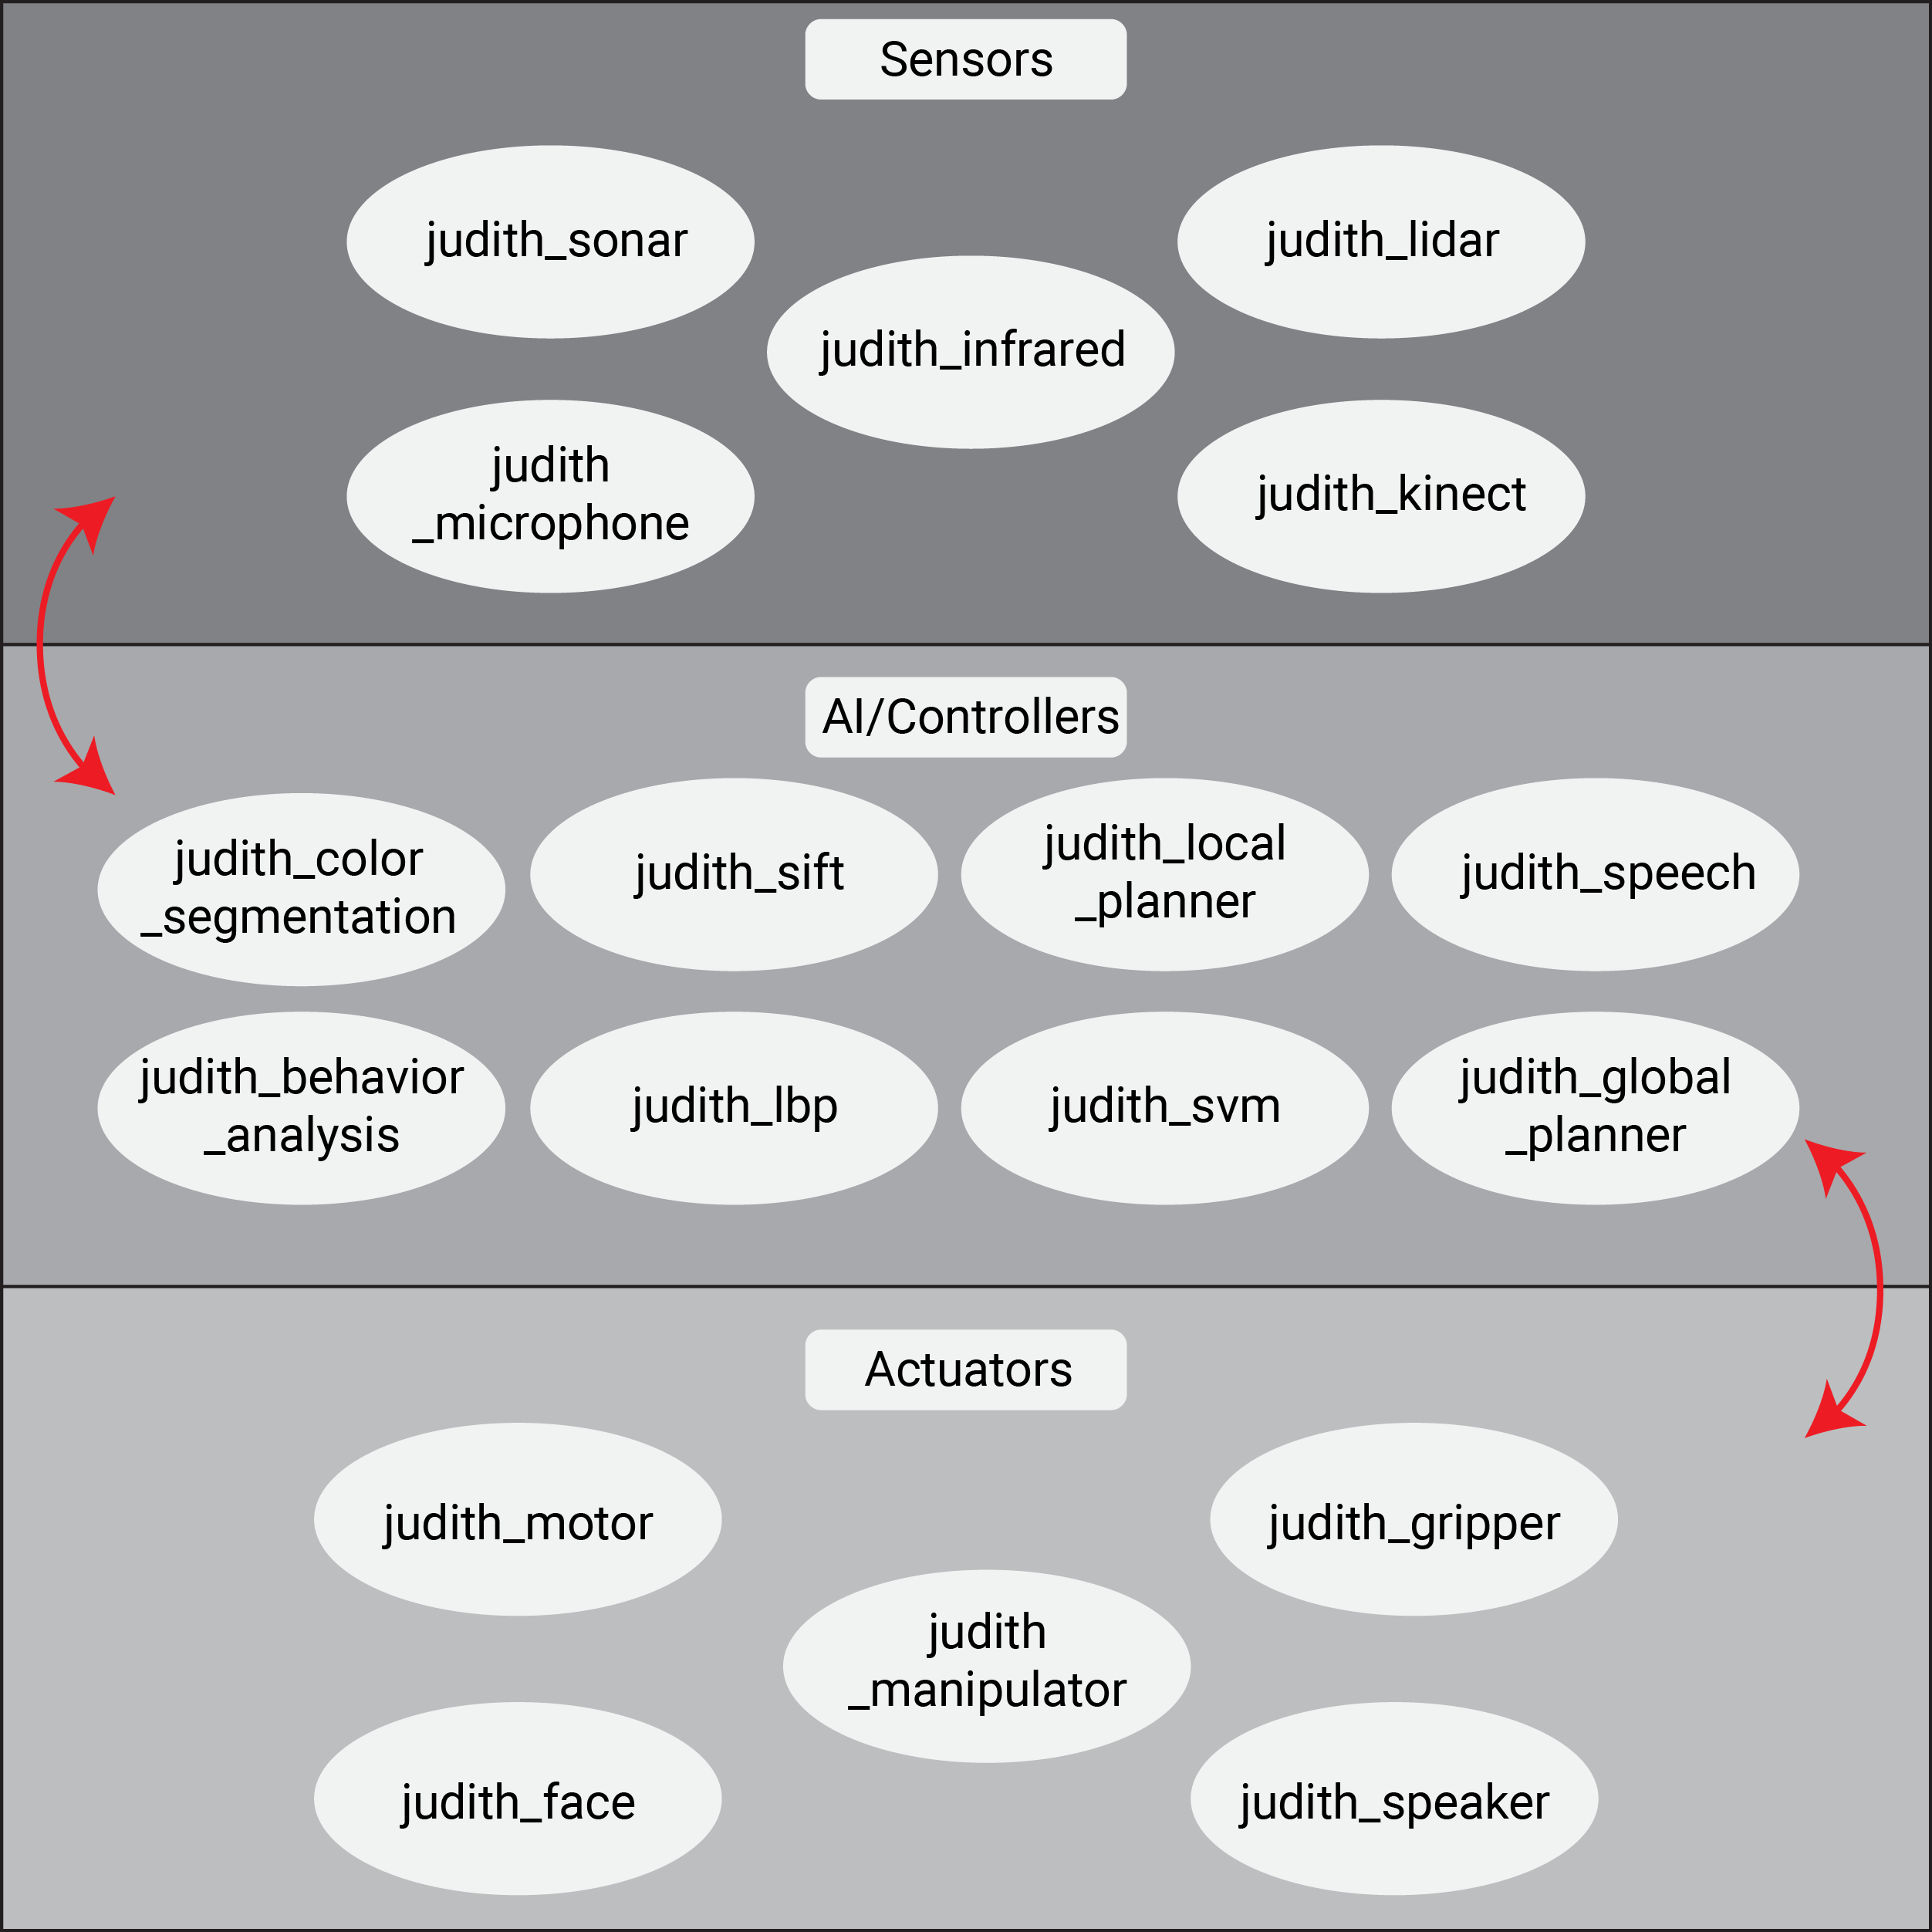
\includegraphics[width = \textwidth]{figures/architecture.png}
    \caption{Software Architecture of Judith}
    \label{fig:architecture}
\end{figure}

Sensors and actuators layers were developed using C++~\cite{stroustrup:1986}, due to hardware drivers communication, except by judith\_face node, which is developed in Java~\cite{joy:2000} language to create an application on Android~\cite{android:2016} Platform. AI/Controllers layer is developed using Python~\cite{vanrossum:2010} as programming language to all algorithms. These decisions were made having in mind the best performance of our robot during task execution and also the training new members to the team.

\subsection{Face and People Recognition}\label{face-people-recognition}
We understand that, in order to make the user's interaction with the robot more comfortable, it is interesting to recognize and treat them by their name. In that way, we developed nodes that can detect and recognize a person by their face. To make it possible, we acquire an image using a camera (Logitech C920 Webcam or Microsoft Kinect X360 RGB camera) and convert the frame into a OpenCV~\cite{bradski:2000} Image Matrix. This information is used as input for the LBP algorithm which has been widely used for face recognition due to its computational performance~\cite{ahonen:2006,yang:2007,shan:2012,ylioinas:2012,samadi:2013}. LBP algorithm may also help on gender, age and facial expression identification which can be useful when developing a robot's adaptive behavior during interaction.

Beyond facial recognition this set of nodes is responsible for following a single person, without external interference during process. To perform this task, three techniques were combined. First is face detection followed by extraction of the color from person t-shirt~\cite{pulli:2012,laganiere:2011,baggio:2012}. With the t-shirt color defined, we perform color segmentation using OpenCV~\cite{kang:2008,oliveira:2009,culjak:2012}. The last technique is skeleton extraction through the Nite/OpenNI library for Microsoft Kinect~\cite{openni:2011}. With this information, the robot can follow the direction of a certain person and also identify the distance between them.

\subsection{Object Detection}\label{object-detection}
Object detection is done by using feature extraction, detection and matching algorithms. A collection of object textures is kept in the robot's memory as bitmap images, each image being part of a class that represents a particular object. When object detection is called for, the robot extracts features from the stored images using either SURF \cite{bay_speeded-up_2008} or SIFT \cite{lowe_object_1999} (the algorithm can be chosen during the robot's startup). Then, it extracts features from the camera feed and matches them with the features from the stored textures. Feature matching is done using brute-force matching: if a certain number of features from a given texture is found in a frame from the camera feed, then a transformation is done to fit the texture in the frame and a rectangle is drawn around the object, identifying it in the frame.

A more efficient object detection procedure is achieved if the robot is able to extract a background image from the environment. This way, the background can be subtract from frames in real time and object detection is only performed in parts of the frame that change.

\subsection{Speech Recognition and Synthesis}\label{speech}
Speech is one of the most important ways to interact with a human. Because of that, we decided to give Judith a female voice, which is generated by the Festival Speech Synthesis System \footnote{\url{http://www.cstr.ed.ac.uk/projects/festival/}}, developed by the University of Edinburg. Additionally, voice commands are used to start all of the robots functions. Speech recognition is made using the CMU Pocketsphinx~\cite{huggins:2006}.

\subsection{Navigation Stack}\label{navigation}
To interact with the environment, the robot needs to know where it is and how to navigate autonomously. In order to do that, Judith creates a map of the environment using the GMapping application and a Hokuyo URG-04LX-UG01 proximity laser. The map is then saved as a bag using a node from ROS called map\_server.

All saved maps can then be used by the robot's simultaneous localization and mapping (SLAM) node. The \emph{Adaptive Monte Carlo Localization} (AMCL) algorithm \cite{fox:1999} uses the maps along with data collected from the laser in real time to make the robot capable to locate its position on the map. With the position known, we are able to give the robot a point to go on the map. It then uses the A* algorithm to make the route between the current position and the desired position. During the completion of the path, it executes a \emph{Dynamic Window Approach}(DWA) algorithm to plan movements locally.

\subsection{Object Manipulation}\label{manipulation}
For manipulating an object, we first use object detection node (see sec.~\ref{object-detection}) to know its current position. The manipulator executes a series of predetermined movements to put the gripper on the robot's view. A PCL algorithm~\cite{aldoma:2012} is then used to segment the gripper and get object distance. In the final step we execute planning to move KUKA youBot arm joints to get the gripper closer and grab the object.

\vspace{-1.25cm}
%\section{Introduction}
%While writing the TDP, please focus on your current research and state clear its scientific contribution value and why it is important for you and the league. The length of the TDP is limited to 8 pages. Please leave the hardware and software description for the end of the paper.
%
%Remember that the TDP must contain the following information:
%
%\begin{itemize}
%	\item Description of the hardware and software including a list of integrated externally available components (including commercial products, freeware, Open Source, etc.)
%	\item Innovative technology and scientific contribution
%	\item Photo(s) of the robot
%	\item Focus of research/research interests
%	\item Re-usability of the system for other research groups
%	\item Applicability of the robot in the real world
%\end{itemize}
%
%\section{Background}
%% We are Buy n Large. We have no competitors so no background is required.
%\lipsum[1-3]
%
%\section{BnL Trash Seeker Algorithm (Main research)}
%\lipsum[4-14]
%
%\section{Experiments and results}
%\lipsum[15-20]
%
%\section{Conclusions and future work}
%\lipsum[21-24]
%
%\section*{Robot WALL-E Hardware Description}
%\textit{(In this section briefly describe the software and hardware of the robot)}
%
%Robot WALL-E has the patented \textit{BnL Optimized Design} for garbage recollection. Specifications are as follows:
%
%%\begin{figure}
%%% \begin{wrapfigure}[13]{r}{0.4\textwidth}
%%	\centering
%%	\includegraphics[width=0.4\textwidth]{images/wall-e.jpg}
%%	\caption{Robot WALL-E}
%%	\label{fig:virbot}
%%% \end{wrapfigure}
%%\end{figure}
%
%
%\begin{itemize}
%	\item Base: BnL all-terrain base (differential pair), 2.5m/s max speed.
%	\item Torso: BnL compressor with solar charger.
%	\item Left and right arms: Mounted on torso. 7 DOF, anthropomorphic, BnL Design. Maximum load: 20kg.
%	\item Neck: BnL telescopic neck with pan and tilt.
%	\item Head: 1DOF BnL Expressive Eyes
%	\item External devices: None
%	\item Robot dimensions: height: 1.2m (max), width: 0.7m depth 0.8m
%	\item Robot weight: 50kg.
%\end{itemize}
%
%\textit{Also our robot incorporates the following devices:}
%
%%\begin{itemize}
%%	\item \BnL Battery charge indicator
%%	\item \BnL Auto-focus all-purpose cameras
%%	\item \BnL 7DOF heavy duty fingers
%%	\item \BnL Cockroach
%%\end{itemize}
%
%\section*{Robot's Software Description}
%Please describe in this section the software you are using to control your robot.
%Consider the following example:
%
%\textit{For our robot we are using the following software:}
%
%\begin{itemize}
%	\item Platform: BnL Operating System
%	\item Navigation, localization and mapping: BnL Navigator
%	\item Face recognition: None. Not designed for human interaction.
%	\item Speech recognition: BnL All-purpose recognizer. Please refer to [1, 2, 3]
%	\item Speech generation: None. Not designed for human interaction.
%	\item Object recognition: BnL Trash Seeker Algorithm. See description on previous sections.
%	\item Arms control and two-hand coordination: BnL automatic controller. Please refer to [4, 5, 6]
%\end{itemize}

%\section*{Bibliography}
\bibliographystyle{unsrt}
\bibliography{refs}
\end{document} 